\chapter{SYSTEM ANALYSIS}
\label{ch:system_analysis}

This chapter documents the empirical analysis of the dataset, data cleaning and preprocessing pipelines, exploratory data visualization, mathematical foundations of the proposed machine learning algorithms, end-to-end project pipeline, multidimensional feasibility study, and execution environment for ClauseIQ. All numerical metrics and distributions presented in this chapter are derived directly from the verified dataset and repository artifacts.

% ----------------------------------------------------------------------
% Section 3.1: Analysis of the Dataset
% ----------------------------------------------------------------------
\section{Analysis of the Dataset}
\label{sec:dataset_analysis}

\subsection{About the Dataset}
\label{subsec:about_dataset}
ClauseIQ is built upon the \textbf{Contract Understanding Atticus Dataset (CUAD)}, an authoritative legal natural language processing benchmark curated by The Atticus Project. CUAD consists of 510 real-world commercial contracts obtained from the United States Securities and Exchange Commission (SEC) EDGAR database. The corpus comprises diverse transactional agreements, including master services agreements, joint venture agreements, licensing pacts, intellectual property assignments, and merger documentation.

In its native distribution, CUAD is packaged in a SQuAD-style JSON format, wherein 41 distinct legal categories are mapped to span-level annotations across full contract documents. To construct a standardized, supervised classification and retrieval engine, these span annotations were extracted, normalized, and flattened into a structured tabular corpus.

The resulting working dataset of ClauseIQ contains \textbf{12,204 rows} structured into three core attributes:
\begin{enumerate}
    \item \texttt{contract\_id} (String): Unique identifier corresponding to the source commercial contract (510 unique contracts).
    \item \texttt{clause\_text} (String): The extracted, operative contractual text span.
    \item \texttt{category} (String): The expert-annotated legal category label (\textbf{41 unique classes}).
\end{enumerate}

Importantly, ClauseIQ models the full, unreduced \textbf{41-class problem space}. The system does not truncate the problem to an arbitrary subset of 8 or 9 classes, thereby preserving the genuine real-world taxonomy and difficulty of enterprise legal review.

\subsection{Explore the Dataset}
\label{subsec:explore_dataset}

\subsubsection*{Dataset Completeness and Missing Values}
Data integrity checks were executed across all 12,204 records in the flattened corpus. As summarized in Table \ref{tab:dataset_schema}, all three attributes exhibit 100\% completeness, with zero missing, null, or undefined values.

\begin{table}[h!]
\centering
\small
\begin{tabular}{lcccc}
\toprule
\textbf{Column Name} & \textbf{Data Type} & \textbf{Total Count} & \textbf{Missing Values} & \textbf{Completeness (\%)} \\
\midrule
\texttt{contract\_id} & String (Categorical) & 12,204 & 0 & 100.0\% \\
\texttt{clause\_text} & String (Text)        & 12,204 & 0 & 100.0\% \\
\texttt{category}    & String (Target)      & 12,204 & 0 & 100.0\% \\
\bottomrule
\end{tabular}
\caption{Dataset schema and missing value analysis ($N = 12,204$)}
\label{tab:dataset_schema}
\end{table}

\subsubsection*{Duplicate and Boilerplate Analysis}
Deduplication analysis revealed zero duplicate rows across the entire dataset. However, text-level analysis identified that \textbf{1,655 clause texts repeat across distinct contracts}, representing 13.56\% of all records, leaving \textbf{10,549 unique distinct clause text strings}. 

In legal contracting, this repetition is an expected domain characteristic rather than an artifact of faulty data collection. Commercial contracts heavily utilize standardized boilerplate covenants (e.g., standard ``\textit{prior written consent}'' stipulations, standard Delaware governing law provisions, or formal notice requirements) across unrelated corporate agreements. Preserving these shared boilerplate provisions is necessary to ensure the classifier learns standard legal phrasing.

\subsubsection*{Contract-Level Clause Distribution}
The 12,204 clauses originate from 510 distinct contracts. The distribution of clauses per contract varies significantly depending on contract complexity, governing structure, and total length:
\begin{itemize}
    \item \textbf{Mean clauses per contract:} 23.93
    \item \textbf{Median clauses per contract:} 19.00
    \item \textbf{Minimum clauses in a contract:} 1
    \item \textbf{Maximum clauses in a contract:} 93
\end{itemize}

Figure \ref{fig:clauses_per_contract} illustrates the distribution of clause counts per contract. While a typical agreement contains between 15 and 30 annotated clauses, complex transaction agreements contain up to 93 distinct provisions.

\begin{figure}[h!]
\centering
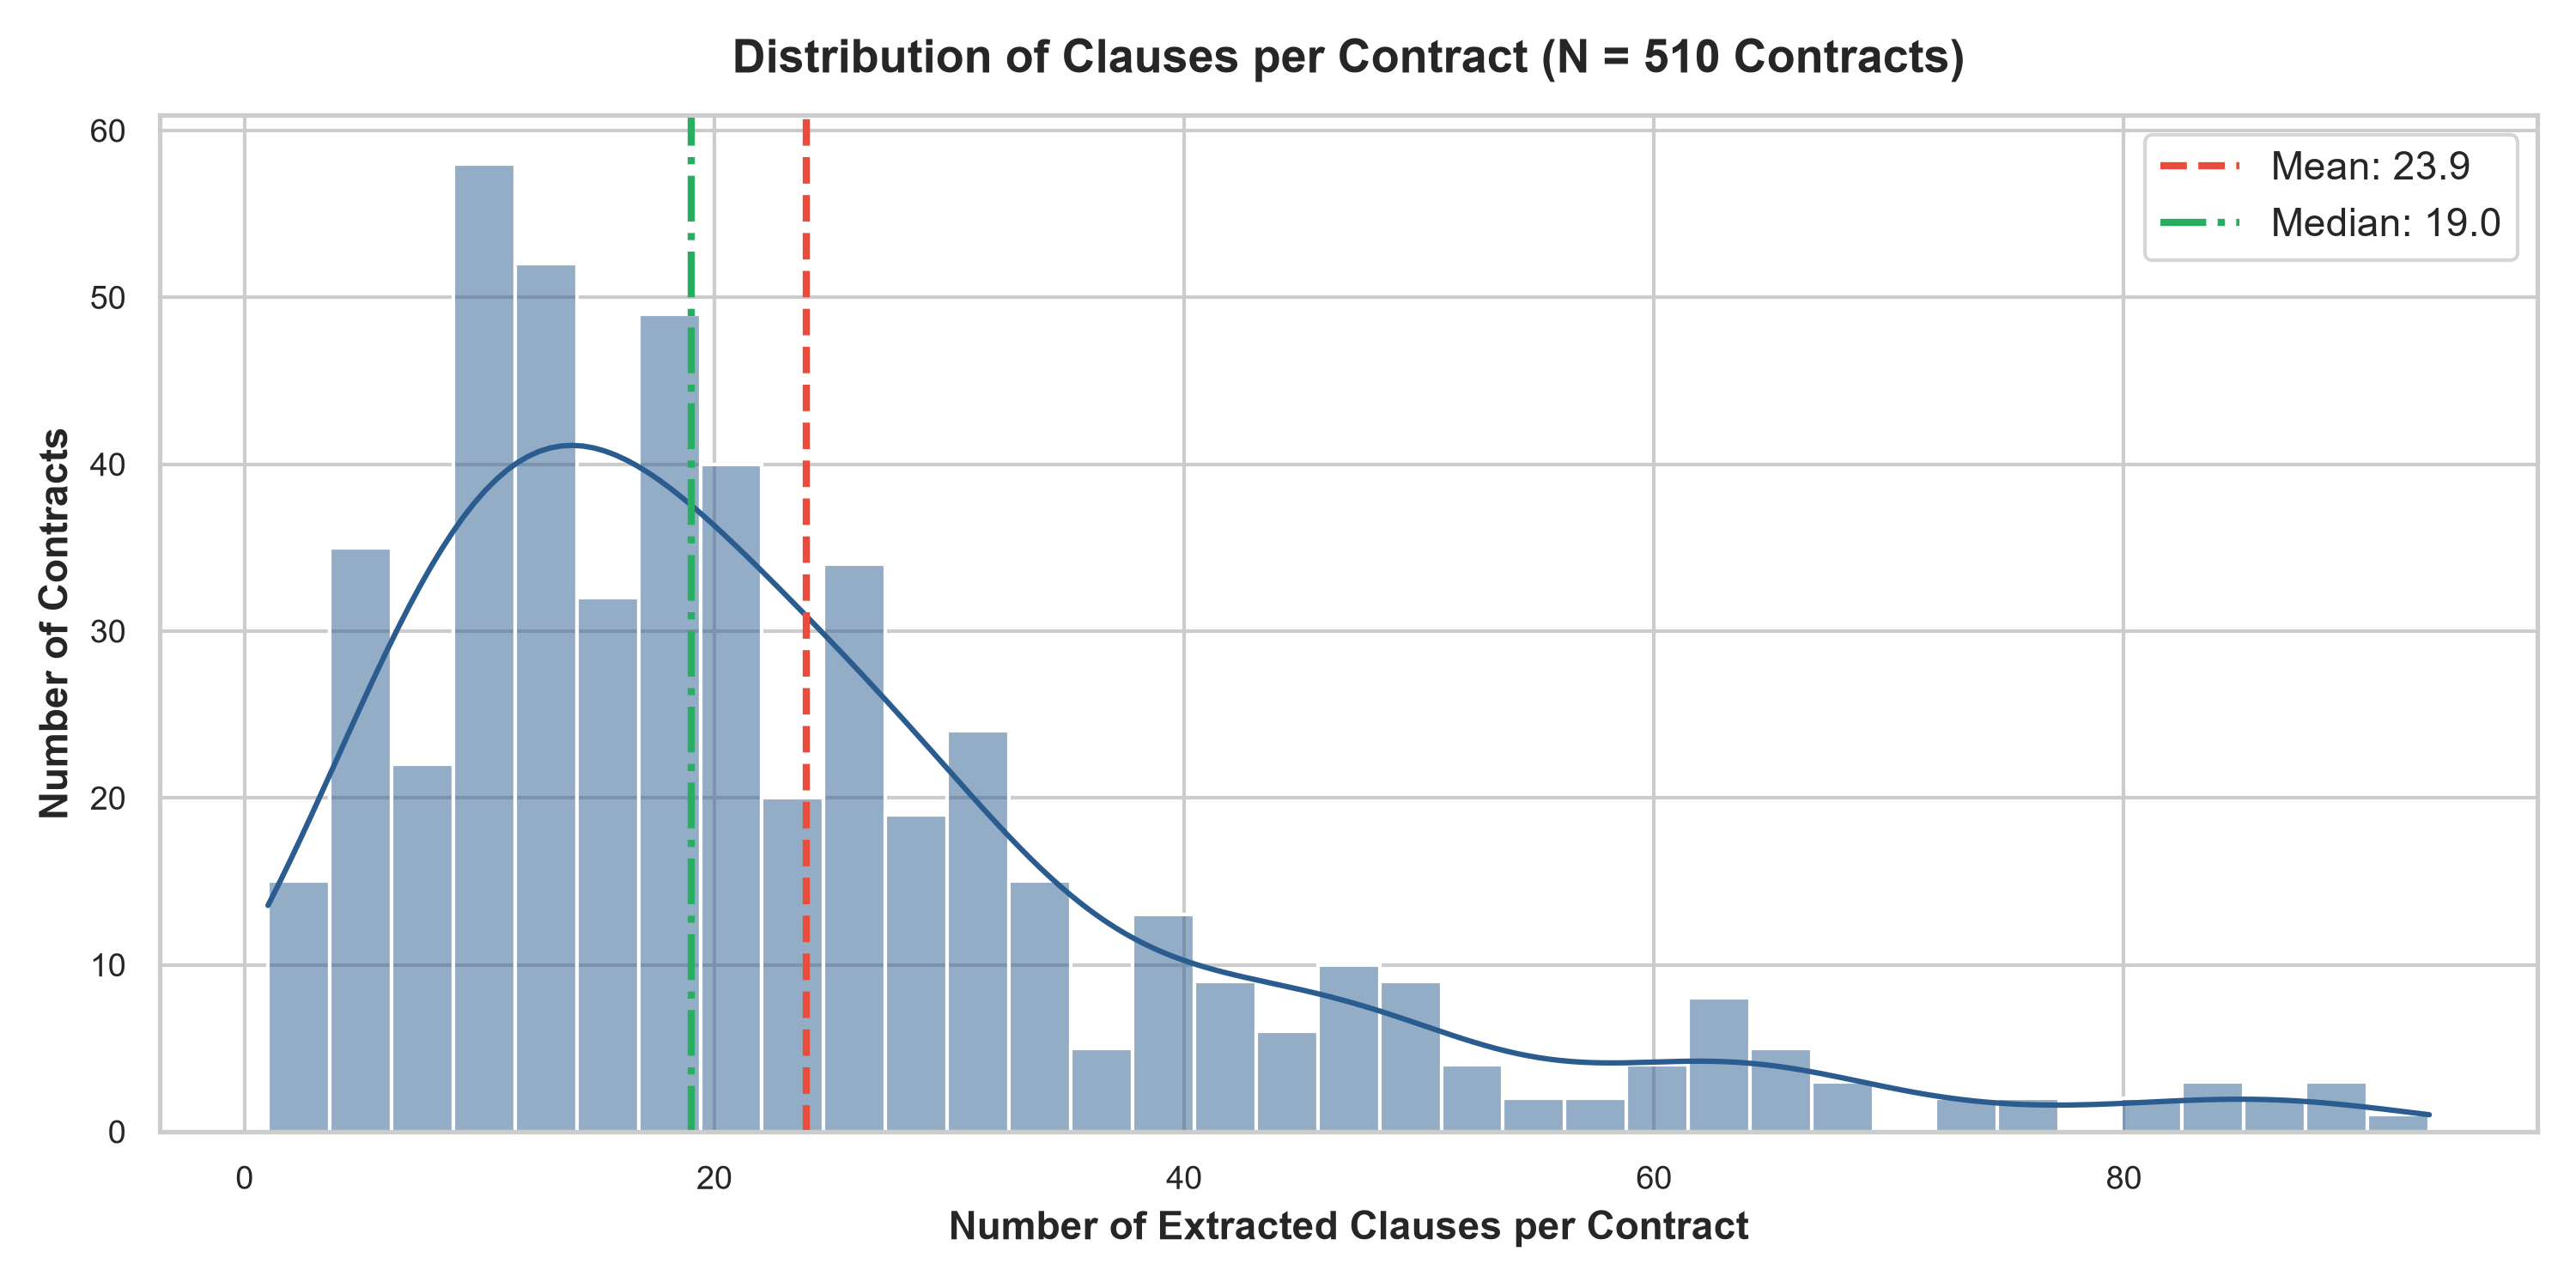
\includegraphics[width=0.85\textwidth]{figures/clauses_per_contract.png}
\caption{Distribution of annotated clauses per contract across 510 CUAD contracts}
\label{fig:clauses_per_contract}
\end{figure}

\subsubsection*{Class Distribution and Severe Imbalance}
The 41 legal categories display extreme class imbalance. Table \ref{tab:class_distribution_extremes} outlines the ten most frequent and five least frequent categories in the dataset.

\begin{table}[h!]
\centering
\small
\begin{tabular}{clcclc}
\toprule
\textbf{Rank} & \textbf{Category (Frequent)} & \textbf{Count} & \textbf{Rank} & \textbf{Category (Rare)} & \textbf{Count} \\
\midrule
1  & Parties                    & 1,251 & 37 & Source Code Escrow         & 67 \\
2  & Cap On Liability           & 742   & 38 & Unlimited/All-You-Can-Eat  & 43 \\
3  & Audit Rights               & 642   & 39 & Non-Disparagement          & 42 \\
4  & Governing Law              & 462   & 40 & Third Party Beneficiary    & 39 \\
5  & Anti-Assignment            & 652   & 41 & Price Restrictions         & 27 \\
\bottomrule
\end{tabular}
\caption{Most frequent vs. least frequent clause categories in ClauseIQ}
\label{tab:class_distribution_extremes}
\end{table}

The largest class, \textit{Parties}, comprises \textbf{1,251 clauses} (10.25\% of the total dataset), whereas the smallest category, \textit{Price Restrictions}, comprises merely \textbf{27 clauses} (0.22\% of the dataset). This establishes an extreme \textbf{class imbalance ratio of 46.33 : 1}. Section \ref{subsec:class_variables} addresses the critical algorithmic and evaluation implications of this distribution.

\subsubsection*{Text Length and Syntactic Statistics}
To quantify the linguistic characteristics of the clauses, three metrics were computed: word count, character length, and sentence count. Table \ref{tab:text_statistics} presents the summary statistics.

\begin{table}[h!]
\centering
\small
\begin{tabular}{lccc}
\toprule
\textbf{Metric} & \textbf{Word Count} & \textbf{Character Length} & \textbf{Sentence Count} \\
\midrule
\textbf{Minimum} & 3      & 9        & 1    \\
\textbf{Maximum} & 479    & 3,169    & 24   \\
\textbf{Mean}    & 45.89  & 289.16   & 1.48 \\
\textbf{Median}  & 36.00  & 228.00   & 1.00 \\
\textbf{Std Dev} & 39.42  & 251.84   & 1.12 \\
\bottomrule
\end{tabular}
\caption{Summary statistics of clause text dimensions ($N = 12,204$)}
\label{tab:text_statistics}
\end{table}

The statistics highlight substantial structural heterogeneity. The shortest valid clauses contain as few as 3 words (e.g., party entities or agreement dates), while expansive indemnification or non-compete clauses span up to 479 words and 24 sentences.

% ----------------------------------------------------------------------
% Section 3.2: Data Preprocessing
% ----------------------------------------------------------------------
\section{Data Preprocessing}
\label{sec:data_preprocessing}

\subsection{Data Cleaning}
\label{subsec:data_cleaning}
To transform raw contractual text into uniform numerical representations suitable for machine learning, a systematic preprocessing pipeline was implemented:
\begin{enumerate}
    \item \textbf{Text Extraction:} Ingestion of contractual text strings from structured CSV and document extractors.
    \item \textbf{Clause Splitting:} Detection of clause boundaries based on paragraph breaks, numbered section headers (e.g., \textit{Section 12.1}, \textit{Article IV}), and terminal punctuation.
    \item \textbf{Case Normalization:} Conversion of all text to lowercase to unify vocabulary (e.g., ``\textit{Shall}'' and ``\textit{shall}'' map to the same token).
    \item \textbf{Special Character and Punctuation Handling:} Removal of extraneous formatting characters (tabs, repeated hyphens, non-ASCII symbols) while preserving standard syntactical punctuation that delineates clauses.
    \item \textbf{Whitespace Consolidation:} Regex-based collapse of irregular whitespace into single space characters.
    \item \textbf{Tokenization and Stopword Filtering:} Word-level tokenization combined with English stopword filtering to eliminate low-information grammatical words without discarding legal connectors.
\end{enumerate}

\subsubsection*{Short-Clause and Long-Clause Preservation Policy}
A critical finding from exploratory data analysis is that \textbf{short clauses are not noise}. Legal contracts inherently contain concise, high-value provisions. For instance, in the CUAD dataset, metadata categories such as \textit{Parties} (mean length: 5.6 words) and \textit{Document Name} (mean length: 4.8 words) frequently contain fewer than 5 words. An automated filter removing spans under 5 words would eliminate \textbf{89.8\% of all Parties records} and \textbf{55.0\% of Document Name records}, severely damaging model training. 

Conversely, long clauses (reaching up to 479 words) represent comprehensive, highly negotiated covenants (e.g., complex \textit{Non-Compete} or \textit{License Grant} terms). Truncating these provisions would strip out essential restrictive qualifications. Therefore, all valid annotated clauses are retained, and \textbf{sublinear term frequency scaling} is introduced during vectorization to mathematically regulate the influence of very long provisions.

\subsection{Analysis of Feature Variables}
\label{subsec:feature_variables}
The primary feature variable is the raw \texttt{clause\_text}. While metadata metrics (word count, character length, sentence count) were engineered during EDA to understand the corpus, they are deliberately excluded from classifier training. Passing clause length as an explicit feature would introduce spurious correlations, as length alone cannot reliably differentiate legal rights.

Textual features are extracted using \textbf{Term Frequency--Inverse Document Frequency (TF-IDF)} with the following verified hyperparameters:
\begin{itemize}
    \item \textbf{Vocabulary Dimension:} Capped at the top \textbf{10,000 features} based on term frequency across the training split.
    \item \textbf{N-gram Range:} $(1, 2)$, capturing both unigrams (individual words) and bigrams (two-word collocations). In legal drafting, compound phrases such as ``\textit{governing law}'', ``\textit{prior written}'', and ``\textit{sole discretion}'' carry distinct legal meaning that individual unigrams cannot convey.
    \item \textbf{Sublinear TF Scaling:} Enabled ($\text{sublinear\_tf} = \text{True}$), replacing raw term frequency $TF$ with $1 + \log(TF)$, preventing long clauses with repetitive words from dominating vector magnitudes.
    \item \textbf{Document Frequency Bounds:} Terms appearing in fewer than 2 documents are excluded to filter out typographical anomalies.
\end{itemize}

\subsection{Analysis of Class Variables}
\label{subsec:class_variables}
The target variable is \texttt{category}, comprising 41 discrete legal classes. In a multi-class dataset exhibiting a 46.33:1 imbalance ratio, standard classification accuracy is a deceptive metric. A naive baseline that uniformly predicts the majority class (\textit{Parties}) would achieve an accuracy score while failing completely to detect critical risk categories such as \textit{Price Restrictions}, \textit{Most Favored Nation}, or \textit{Source Code Escrow}.

To ensure that rare categories receive equal optimization priority during model selection, the project adopts \textbf{Macro-Averaged F1-Score (Macro-F1)} as the primary evaluation metric:
\begin{equation}
    \text{Macro-F1} = \frac{1}{C} \sum_{c=1}^{C} F1_c
\end{equation}
where $C = 41$. Macro-F1 calculates the harmonic mean of precision and recall for each category independently and then computes their unweighted arithmetic mean. Under this formulation, correctly classifying a rare \textit{Price Restrictions} clause is weighted identically to classifying a frequent \textit{Parties} clause. Furthermore, class weighting ($\text{class\_weight} = \text{'balanced'}$) is applied to penalize misclassifications in minority classes proportionally to their inverse class frequencies.

% ----------------------------------------------------------------------
% Section 3.3: Data Visualization
% ----------------------------------------------------------------------
\section{Data Visualization}
\label{sec:data_visualization}

\subsection{Category Frequency Distribution}
Figure \ref{fig:class_distribution} displays the frequency distribution across all 41 legal categories in the ClauseIQ dataset. The extreme long-tail distribution visually confirms the severe imbalance, with the top 5 categories accounting for more than 30\% of the entire corpus.

\begin{figure}[h!]
\centering
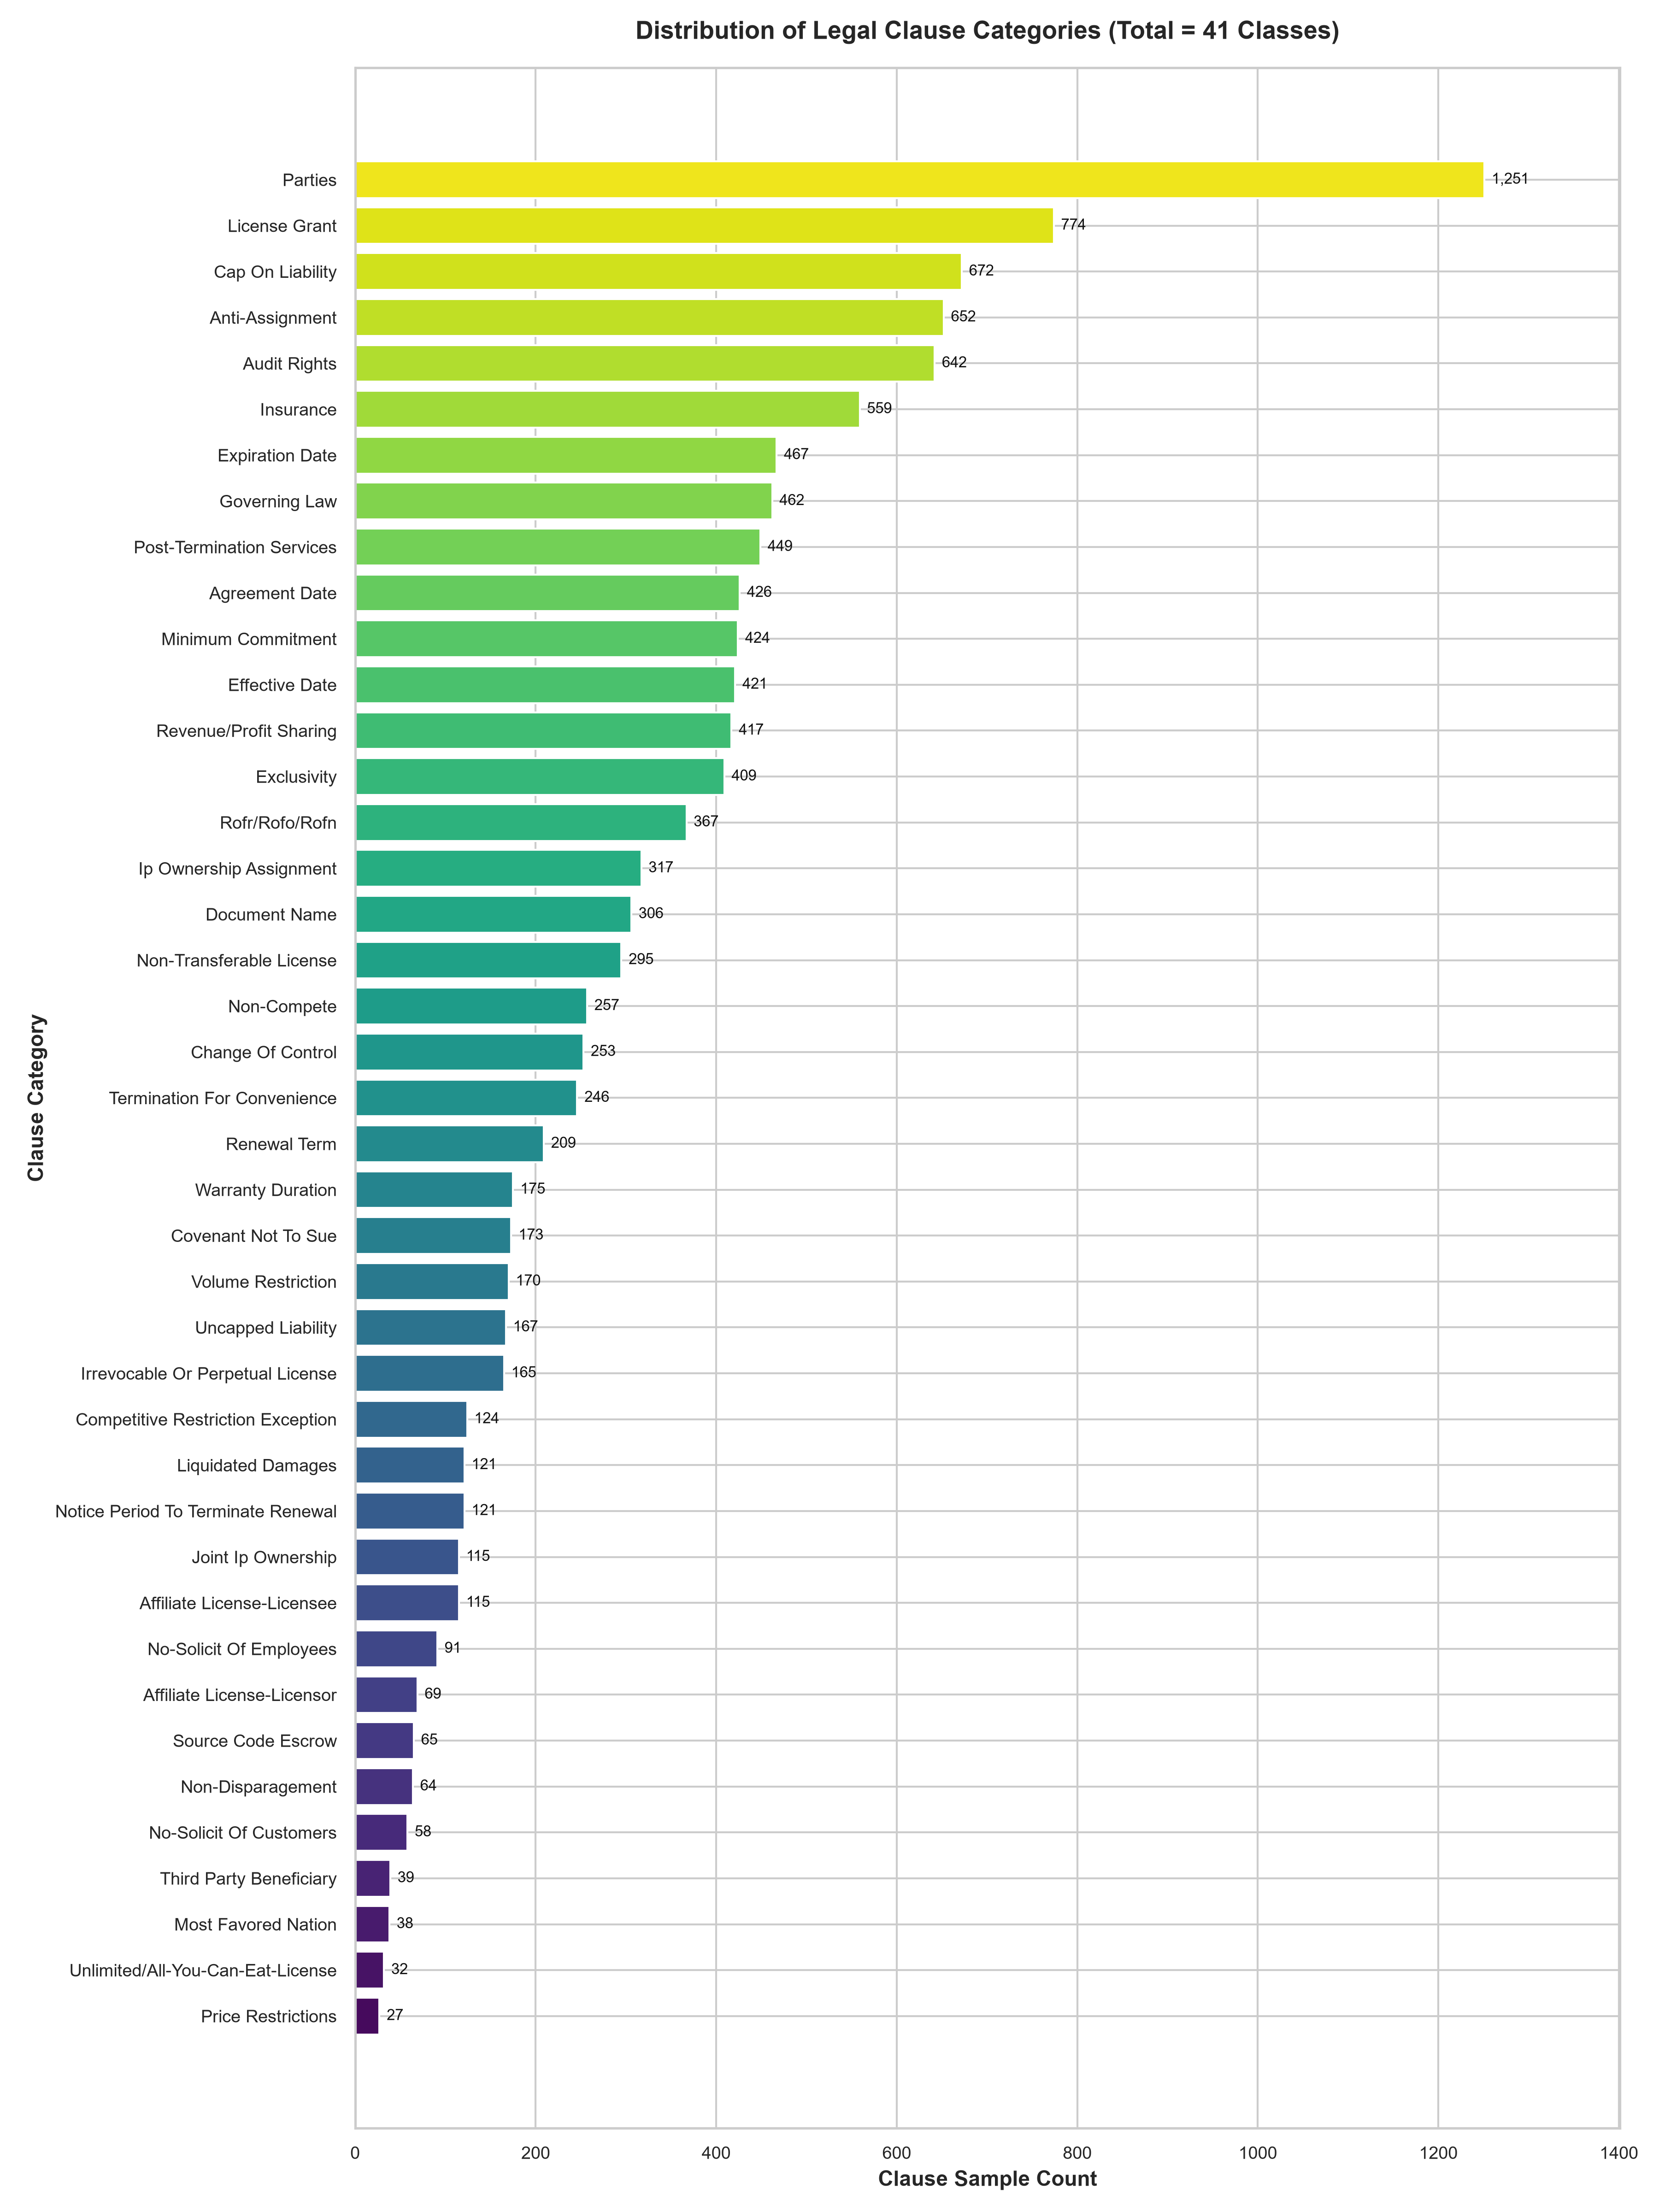
\includegraphics[width=0.92\textwidth]{figures/class_distribution.png}
\caption{Complete 41-category class distribution in the ClauseIQ dataset ($N = 12,204$)}
\label{fig:class_distribution}
\end{figure}

\subsection{Average Clause Word Count by Category}
Figure \ref{fig:avg_word_count} depicts the mean word count across categories. Factual metadata categories (\textit{Agreement Date}, \textit{Parties}) average under 6 words, whereas substantive covenants (\textit{Affiliate License-Licensor}, \textit{Irrevocable Or Perpetual License}) average between 80 and 95 words per clause.

\begin{figure}[h!]
\centering
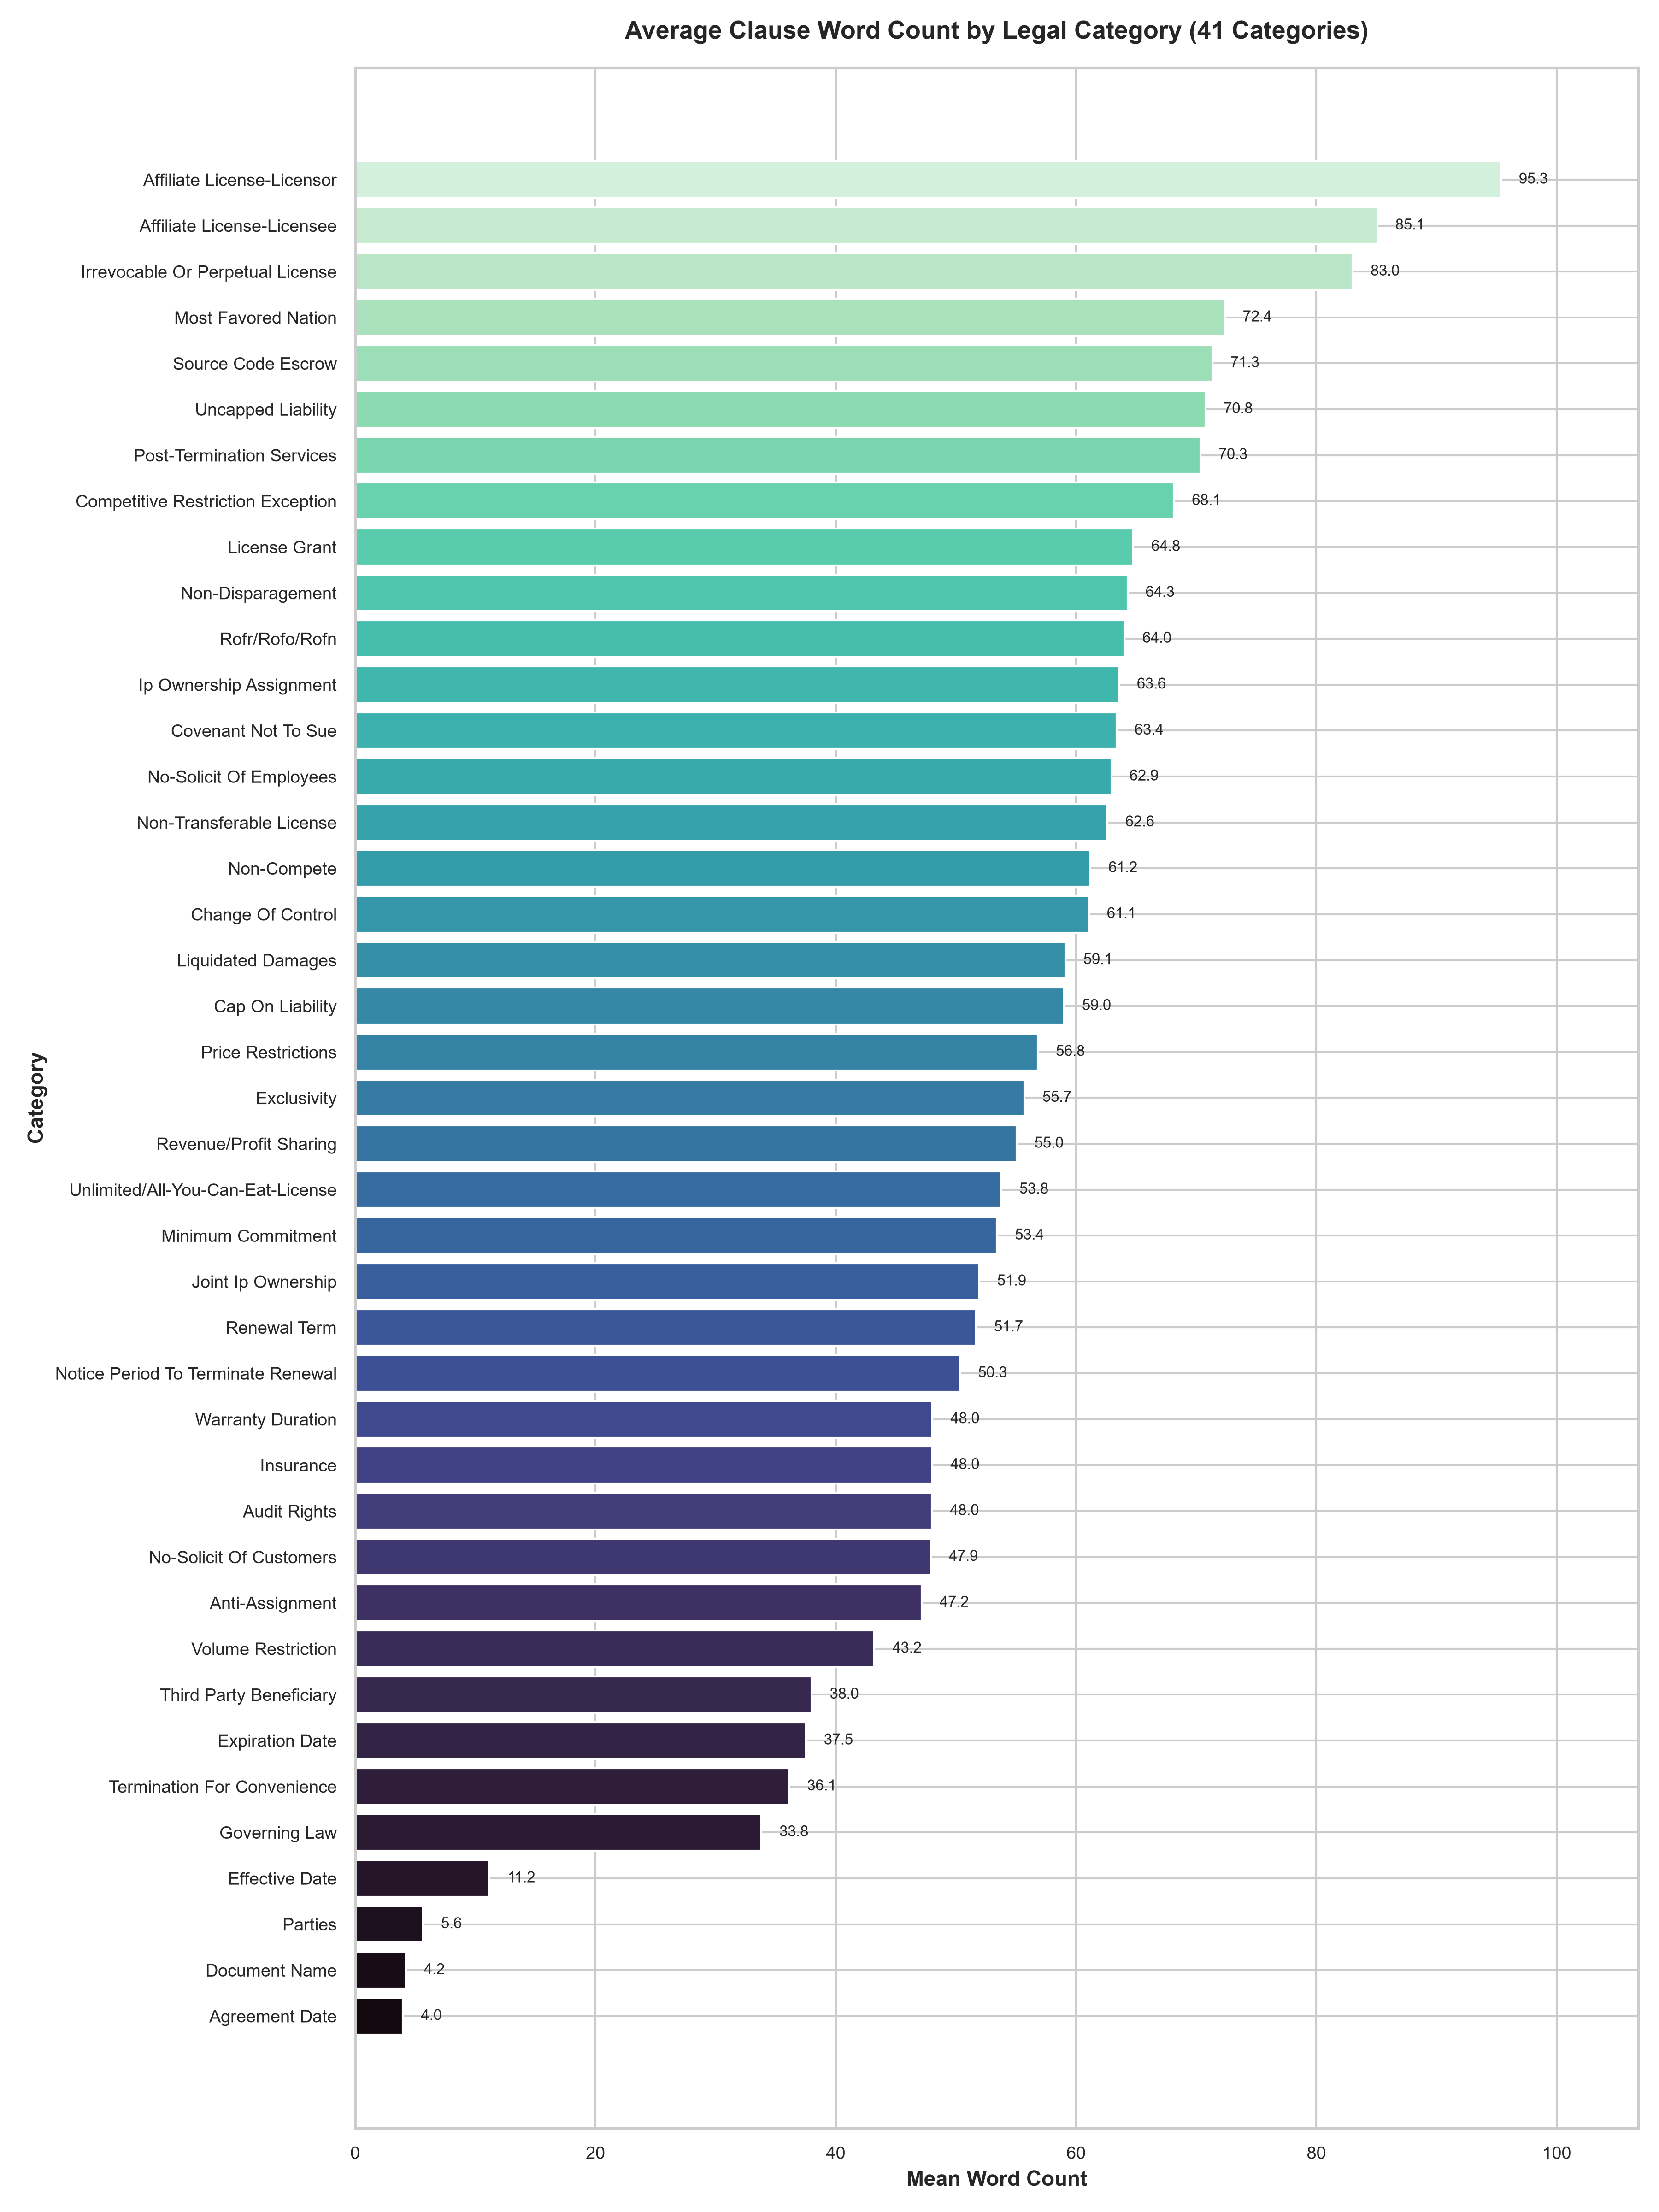
\includegraphics[width=0.92\textwidth]{figures/average_word_count_by_category.png}
\caption{Average clause word count across legal categories}
\label{fig:avg_word_count}
\end{figure}

\subsection{Word Count Distribution and Correlation Heatmap}
Figure \ref{fig:word_count_distribution} shows the right-skewed distribution of clause word counts across the dataset, with a sharp concentration between 15 and 50 words.

\begin{figure}[h!]
\centering
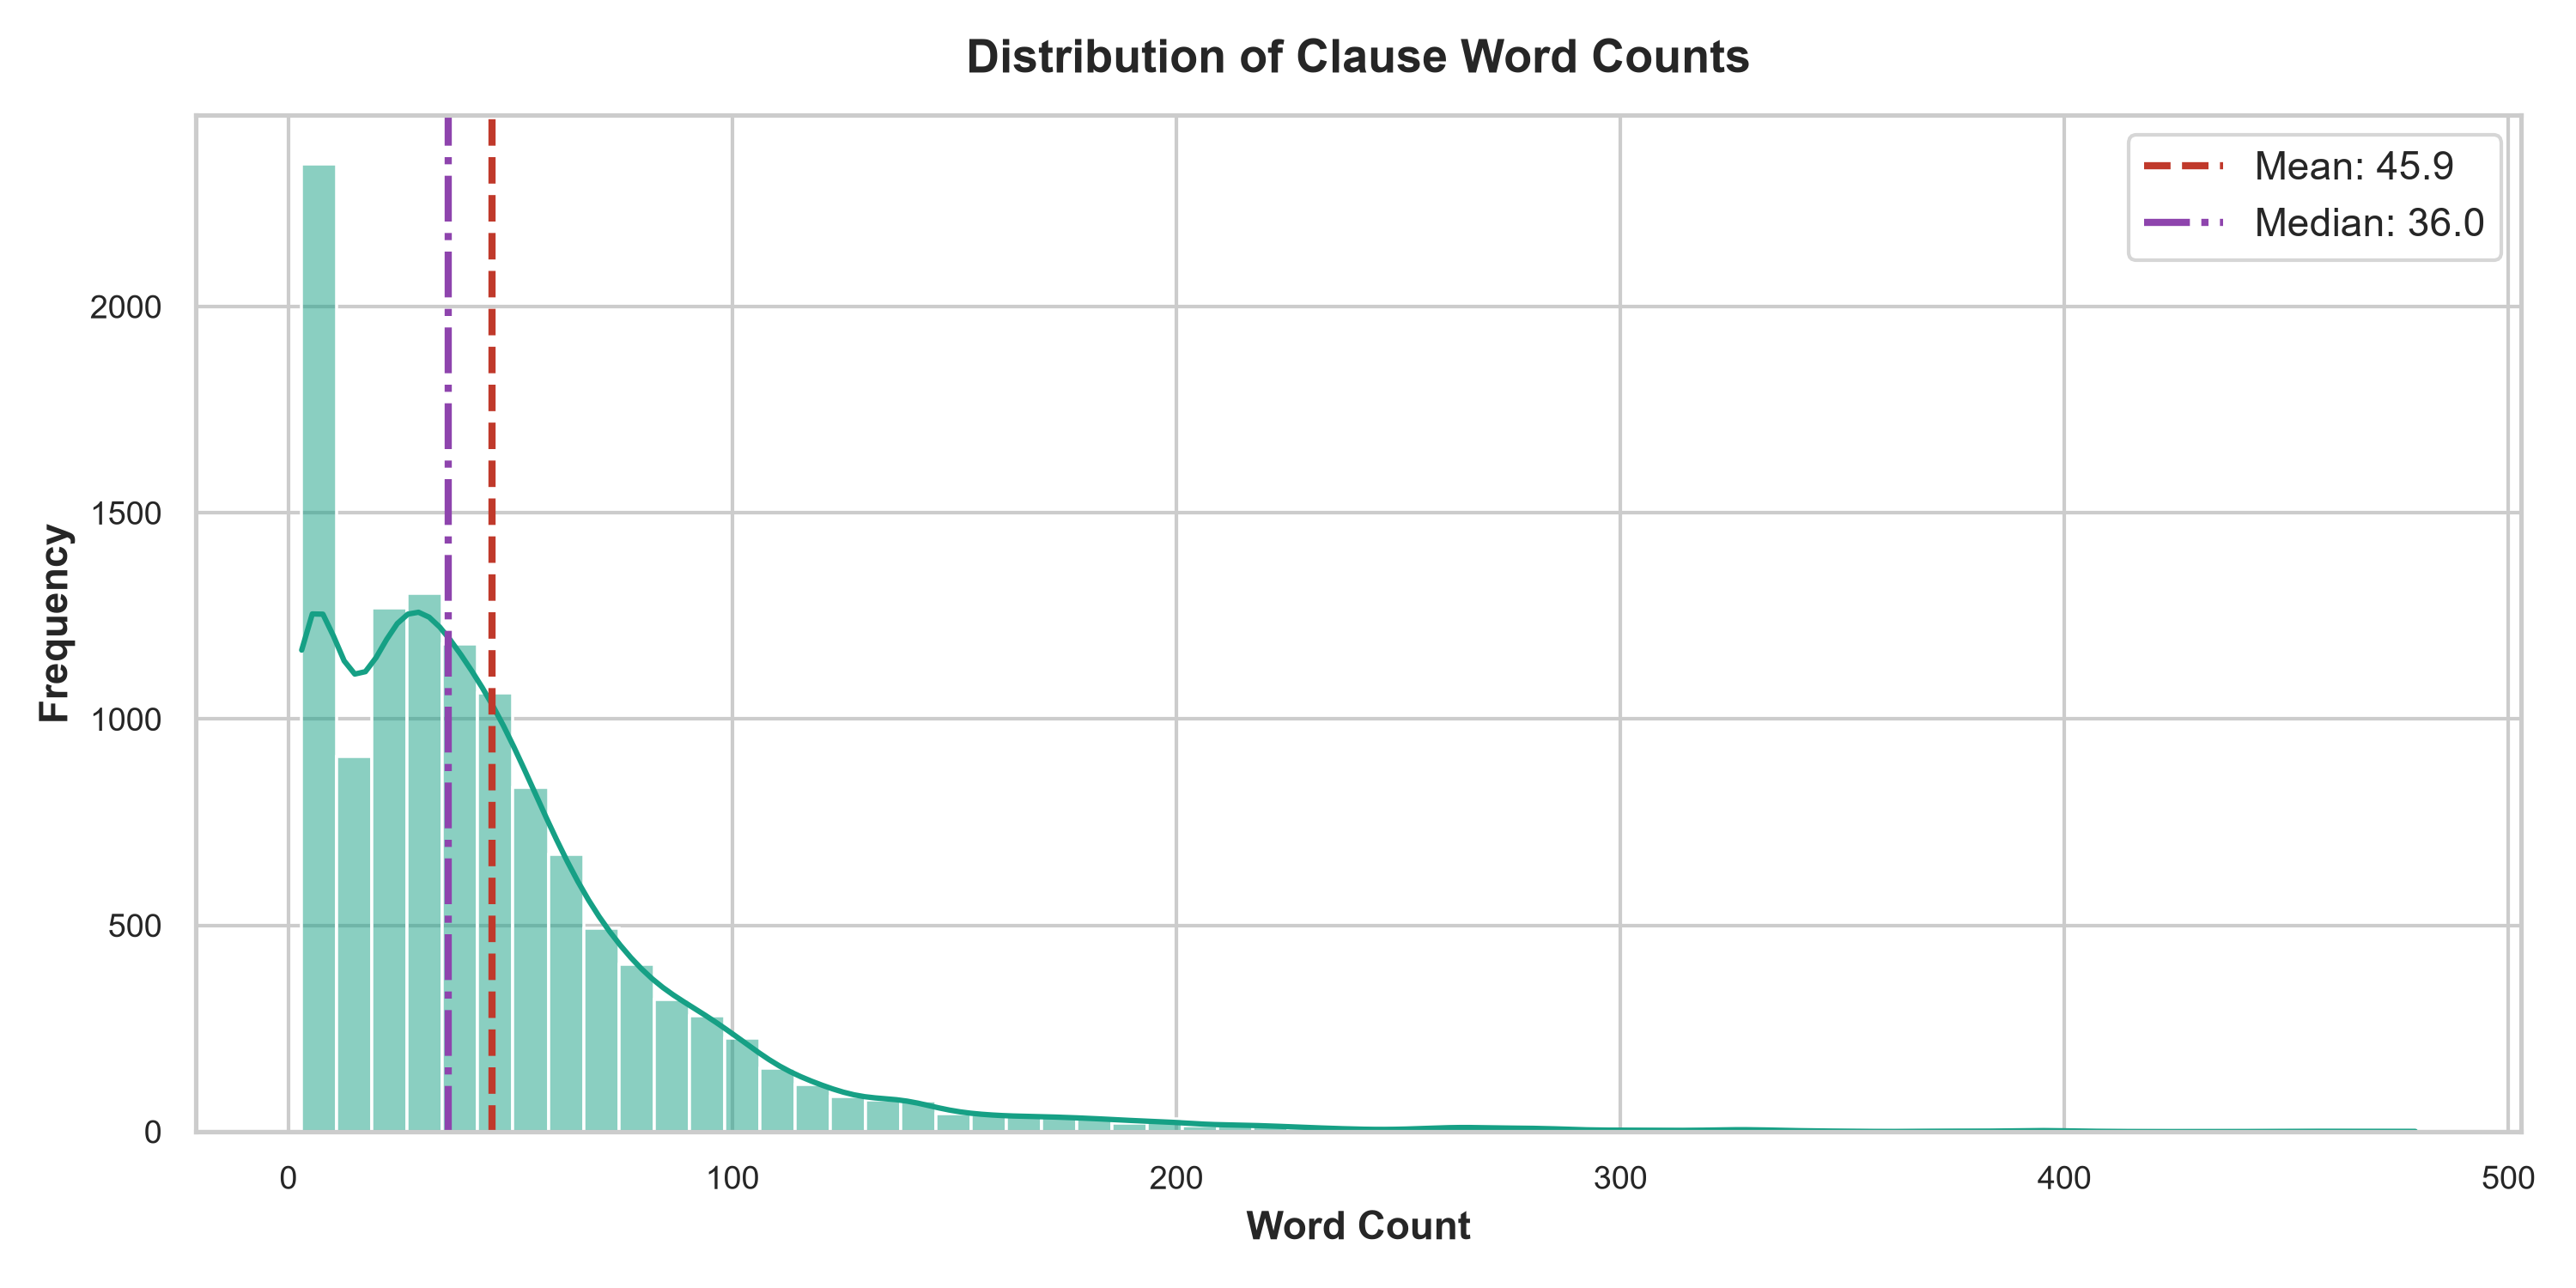
\includegraphics[width=0.85\textwidth]{figures/word_count_distribution.png}
\caption{Distribution of clause word counts}
\label{fig:word_count_distribution}
\end{figure}

Figure \ref{fig:correlation_heatmap} demonstrates the correlation matrix among length metrics; character length and word count display a near-perfect correlation of \textbf{0.9945}, confirming that character length provides no independent discriminatory signal beyond word count.

\begin{figure}[h!]
\centering
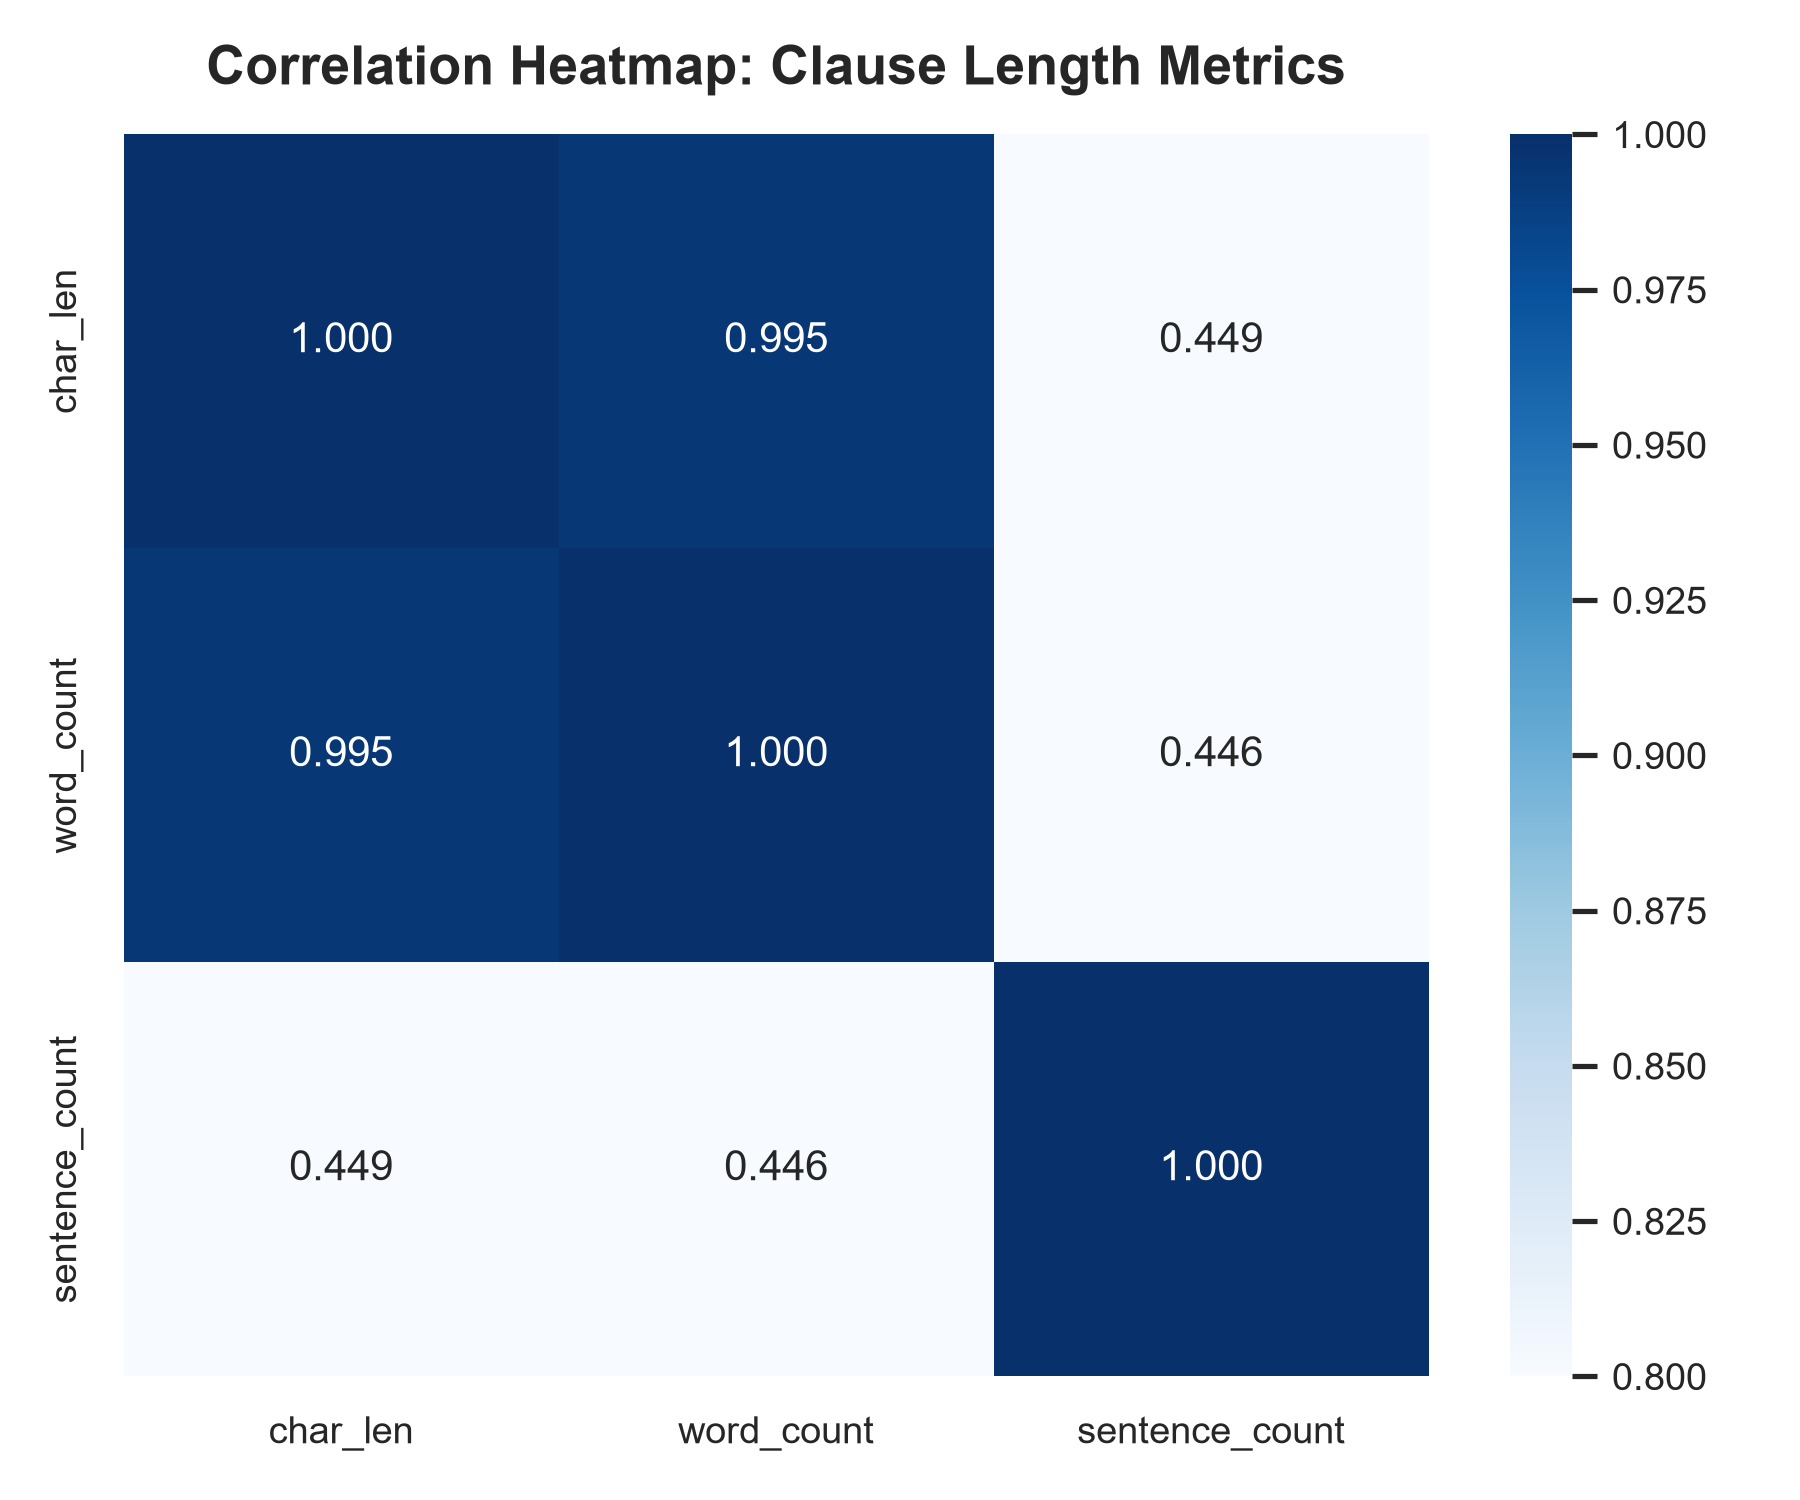
\includegraphics[width=0.85\textwidth]{figures/numerical_correlation.png}
\caption{Correlation matrix of text metrics}
\label{fig:correlation_heatmap}
\end{figure}

\subsection{Top Legal Bigrams}
Figure \ref{fig:top_bigrams} highlights the top 20 most frequent bigrams extracted from the corpus. Standard legal collocations—such as ``\textit{agreement shall}'', ``\textit{set forth}'', ``\textit{effective date}'', and ``\textit{prior written}''—dominate the feature space, justifying the use of bigram feature representations.

\begin{figure}[h!]
\centering
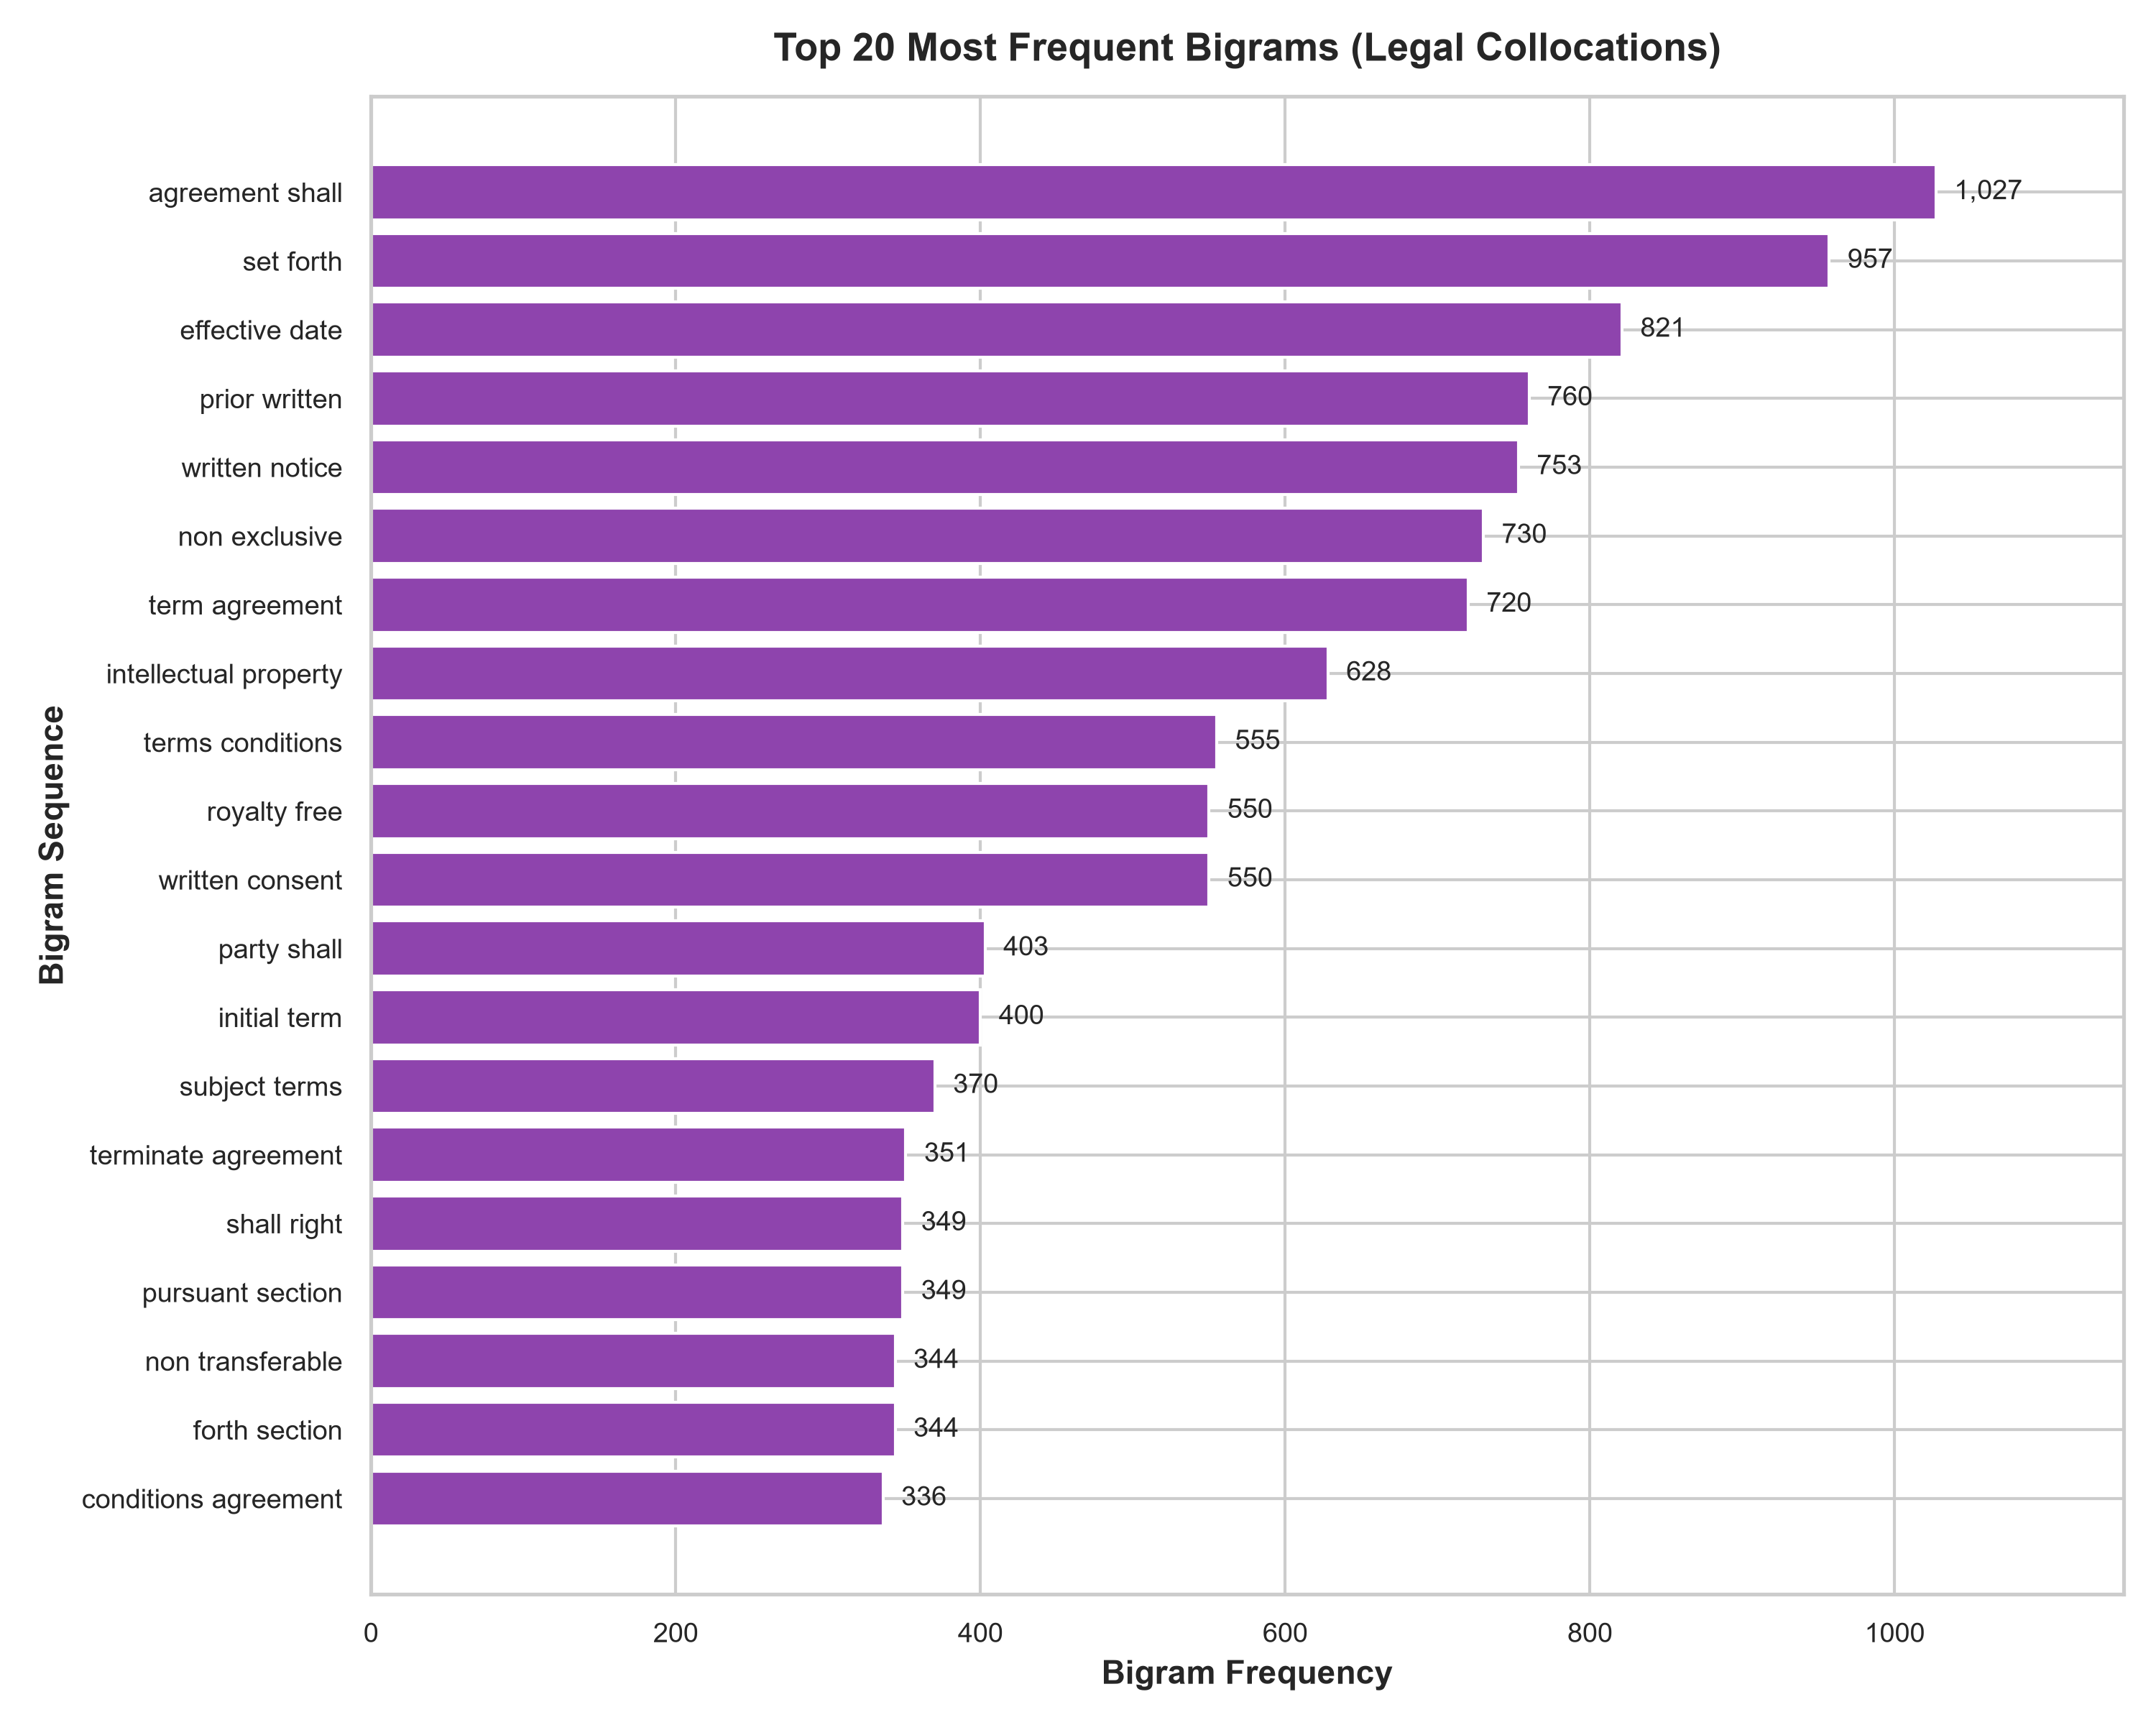
\includegraphics[width=0.85\textwidth]{figures/top_bigrams.png}
\caption{Top 20 most frequent bigrams in the ClauseIQ clause corpus}
\label{fig:top_bigrams}
\end{figure}

% ----------------------------------------------------------------------
% Section 3.4: Analysis of Architecture and(or) Algorithms
% ----------------------------------------------------------------------
\section{Analysis of Architecture and(or) Algorithms}
\label{sec:algorithms_analysis}

\subsection{Detailed Study Report of the Proposed Algorithm(s)}
\label{subsec:proposed_algorithms}
ClauseIQ unites a unified 10,000-dimensional TF-IDF vector space with four classical machine learning classifiers for automated clause categorization, and a vector similarity retrieval module for intelligent clause search.

\subsubsection*{1. TF-IDF Vectorization}
Term Frequency--Inverse Document Frequency converts unstructured text strings into normalized, sparse numerical vectors. 

The Term Frequency ($TF$) represents the normalized frequency of term $t$ in clause $d$:
\begin{equation}
    TF(t, d) = \frac{f_{t,d}}{\sum_{t' \in d} f_{t',d}}
\end{equation}
Under sublinear scaling, this is modified to $1 + \log(f_{t,d})$ for all $f_{t,d} > 0$.

The Inverse Document Frequency ($IDF$) measures the relative specificity of term $t$ across the entire corpus $D$ of $N$ clauses:
\begin{equation}
    IDF(t, D) = \log \left( \frac{1 + N}{1 + DF(t)} \right) + 1
\end{equation}
where $DF(t)$ is the number of clauses containing term $t$.

The composite TF-IDF score is computed as:
\begin{equation}
    TF\text{-}IDF(t, d, D) = TF(t, d) \times IDF(t, D)
\end{equation}
Each resulting vector is subsequently $L_2$-normalized:
\begin{equation}
    v_{\text{norm}} = \frac{v}{\|v\|_2}
\end{equation}

\subsubsection*{2. Multinomial Naive Bayes}
Multinomial Naive Bayes is a probabilistic classifier based on Bayes' theorem under the conditional independence assumption among features given the class label.

Given a feature vector $x = (t_1, t_2, \dots, t_n)$ representing a clause, the posterior probability of category $c$ is:
\begin{equation}
    P(c \mid x) \propto P(c) \prod_{i=1}^{n} P(t_i \mid c)^{f_i}
\end{equation}
where $P(c)$ is the prior probability of category $c$, and $P(t_i \mid c)$ is the probability of term $t_i$ occurring in category $c$.

To eliminate zero-probability errors for unseen terms, Lidstone/Laplace smoothing with parameter $\alpha$ is applied:
\begin{equation}
    P(t_i \mid c) = \frac{N_{ci} + \alpha}{N_c + \alpha |V|}
\end{equation}
where $N_{ci}$ is the sum of TF-IDF weights for term $t_i$ in class $c$, $N_c$ is the total sum across all vocabulary terms for class $c$, and $|V| = 10,000$.

\subsubsection*{3. Linear Support Vector Machine (Linear SVM)}
Support Vector Machines construct optimal separating hyperplanes that maximize the functional margin between classes in high-dimensional feature space. Linear SVM is exceptionally effective for sparse text classification where the feature dimensionality is large.

For multi-class classification across 41 categories, a One-vs-Rest (OvR) formulation is employed, training 41 binary linear classifiers. The primal optimization problem for each binary sub-problem is:
\begin{equation}
    \min_{w, b, \xi} \frac{1}{2} \|w\|^2 + C \sum_{i=1}^{m} \xi_i
\end{equation}
subject to the margin constraints:
\begin{equation}
    y_i (w^T x_i + b) \ge 1 - \xi_i, \quad \xi_i \ge 0, \quad \forall i \in \{1, \dots, m\}
\end{equation}
where $w$ is the normal weight vector, $b$ is the bias offset, $\xi_i$ are slack variables permitting soft-margin misclassifications, and $C$ is the regularization parameter governing the trade-off between margin width and training error.

\subsubsection*{4. Logistic Regression}
Logistic Regression is a discriminative linear model that predicts posterior class probabilities using the multinomial softmax function.

For a clause vector $x \in \mathbb{R}^{10000}$, the probability that it belongs to category $c \in \{1, \dots, 41\}$ is parameterized as:
\begin{equation}
    P(y = c \mid x) = \frac{\exp(w_c^T x + b_c)}{\sum_{j=1}^{41} \exp(w_j^T x + b_j)}
\end{equation}
where $w_c$ and $b_c$ denote the learned weights and intercept for class $c$.

The model parameters are optimized by minimizing the $L_2$-regularized cross-entropy loss across $m$ training samples:
\begin{equation}
    \mathcal{L}(W) = - \sum_{i=1}^{m} \sum_{c=1}^{41} \mathbb{I}(y_i = c) \log P(y_i = c \mid x_i) + \frac{1}{2C} \sum_{c=1}^{41} \|w_c\|_2^2
\end{equation}
Logistic Regression provides class probability estimates through its multinomial softmax formulation, enabling the generation of prediction confidence scores.

\subsubsection*{5. Random Forest Classifier}
Random Forest is an ensemble learning method that constructs a multitude of decision trees during training and outputs the majority voting class among individual trees.

To inject diversity and prevent overfitting on high-dimensional text vectors:
\begin{enumerate}
    \item \textbf{Bootstrap Aggregation (Bagging):} Each decision tree $T_b$ is trained on an independently drawn bootstrap sample of the training dataset.
    \item \textbf{Random Feature Subspaces:} At each internal split node, a random subset of features $\sqrt{|V|}$ is evaluated rather than the entire 10,000-dimensional feature space.
\end{enumerate}

Split quality is evaluated using the Gini Impurity metric:
\begin{equation}
    \text{Gini}(D) = 1 - \sum_{c=1}^{41} p_c^2
\end{equation}
where $p_c$ is the proportion of samples belonging to class $c$ in node $D$. The final ensemble prediction is obtained by majority vote:
\begin{equation}
    \hat{y} = \arg\max_c \sum_{b=1}^{B} \mathbb{I}(T_b(x) = c)
\end{equation}

\subsubsection*{6. Cosine Similarity (Intelligent Search)}
For the intelligent search engine, user queries and contract clauses are embedded into the same 10,000-dimensional TF-IDF vector space. The relevance of a candidate clause vector $B$ to a search query vector $A$ is quantified by calculating the cosine of the angle between them:
\begin{equation}
    \text{Similarity}(A, B) = \cos(\theta) = \frac{A \cdot B}{\|A\|_2 \|B\|_2} = \frac{\sum_{i=1}^{10000} A_i B_i}{\sqrt{\sum_{i=1}^{10000} A_i^2} \sqrt{\sum_{i=1}^{10000} B_i^2}}
\end{equation}

Because both query and clause vectors are $L_2$-normalized during vectorization ($\|A\|_2 = \|B\|_2 = 1$), the cosine similarity simplifies to the efficient sparse dot product:
\begin{equation}
    \text{Similarity}(A, B) = A \cdot B = \sum_{i=1}^{10000} A_i B_i
\end{equation}
Cosine similarity is strictly scale-invariant, preventing longer clauses from receiving artificially elevated scores purely due to document length.

\subsubsection*{7. Performance Evaluation Metrics}
To assess classification performance objectively, standard evaluation metrics are computed on the held-out test split:
\begin{itemize}
    \item \textbf{Precision ($P_c$):} $\frac{TP_c}{TP_c + FP_c}$ (Proportion of predicted class $c$ clauses that are correct).
    \item \textbf{Recall ($R_c$):} $\frac{TP_c}{TP_c + FN_c}$ (Proportion of actual class $c$ clauses correctly identified).
    \item \textbf{Accuracy:} $\frac{\sum_{c=1}^{41} TP_c}{N_{\text{total}}}$ (Overall percentage of correct predictions across all samples).
    \item \textbf{Class F1-Score ($F1_c$):} $2 \times \frac{P_c \times R_c}{P_c + R_c}$ (Harmonic mean of precision and recall for class $c$).
    \item \textbf{Macro-F1:} $\frac{1}{41} \sum_{c=1}^{41} F1_c$ (\textbf{Primary selection metric}; weights all 41 categories equally).
    \item \textbf{Weighted-F1:} $\sum_{c=1}^{41} \left( \frac{N_c}{N_{\text{total}}} \right) F1_c$ (Weights F1 by category sample proportion).
\end{itemize}

\noindent\textbf{Critical Conceptual Distinction:} Macro-F1 is an aggregate classification performance metric calculated over an evaluation dataset. It is not a probability, confidence score, or indicator of the likelihood of an individual prediction. Logistic Regression provides class probability estimates through its multinomial softmax formulation. These probability estimates are distinct from the Macro-F1 evaluation metric.

% ----------------------------------------------------------------------
% Section 3.5: Project Pipeline
% ----------------------------------------------------------------------
\section{Project Pipeline}
\label{sec:project_pipeline}
Figure \ref{fig:project_pipeline} illustrates the multi-stage operational pipeline of ClauseIQ.

\begin{figure}[h!]
\centering
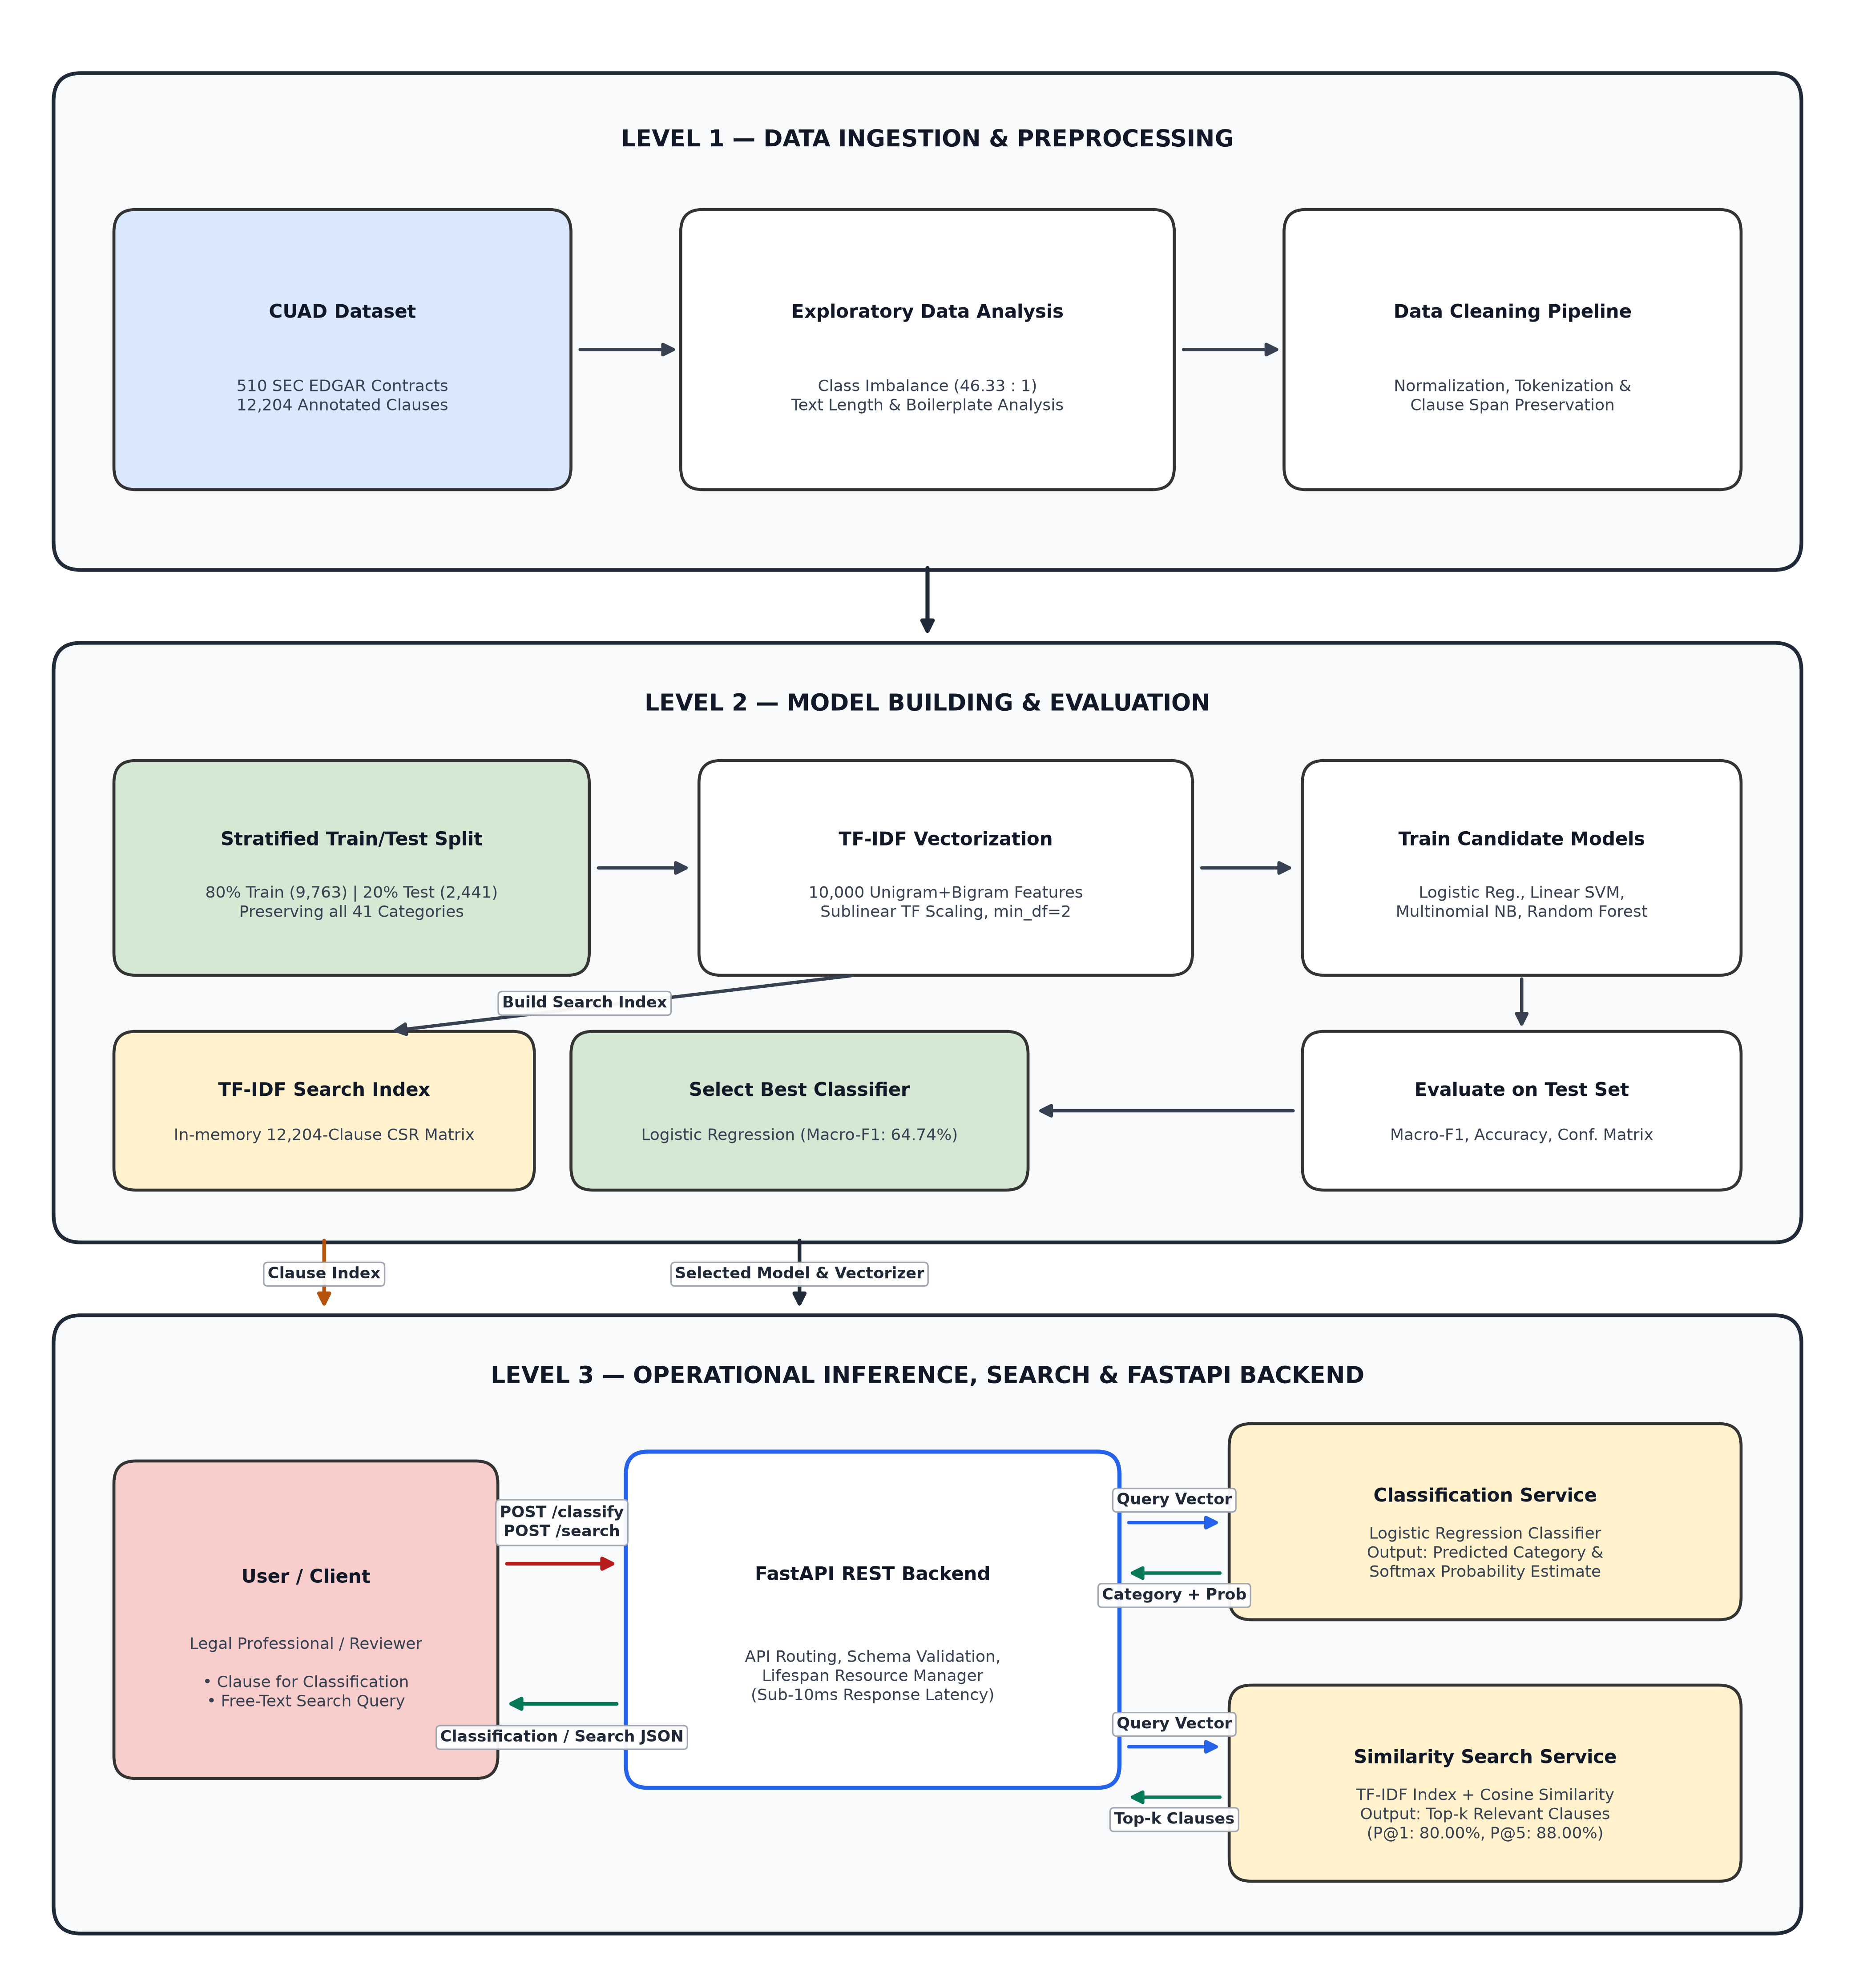
\includegraphics[width=0.85\textwidth]{figures/project_pipeline.png}
\caption{End-to-end ClauseIQ system pipeline architecture}
\label{fig:project_pipeline}
\end{figure}

The pipeline executes through structured operational stages:
\begin{enumerate}
    \item \textbf{Data Ingestion \& Flattening:} Raw CUAD contract JSON annotations are ingested and flattened into a structured tabular schema with 12,204 rows and 41 classes.
    \item \textbf{Data Cleaning \& Stratification:} Normalization, tokenization, and stratified 80/20 train/test splitting ($N_{\text{train}} = 9,763$, $N_{\text{test}} = 2,441$).
    \item \textbf{Feature Extraction:} Fitting of the 10,000-feature unigram+bigram TF-IDF vectorizer with sublinear scaling on the training split.
    \item \textbf{Model Training \& Tuning:} Training and cross-validated tuning of four classical machine learning classifiers.
    \item \textbf{Evaluation \& Selection:} Comprehensive multi-metric benchmark on the held-out test split to identify the optimal production classifier based on Macro-F1.
    \item \textbf{Search Indexing:} Construction of an in-memory sparse CSR vector index over all 12,204 clauses for sub-10ms Cosine Similarity retrieval.
    \item \textbf{API Serving:} Packaging model artifacts and the search engine inside FastAPI REST endpoints.
\end{enumerate}

% ----------------------------------------------------------------------
% Section 3.6: Feasibility Analysis
% ----------------------------------------------------------------------
\section{Feasibility Analysis}
\label{sec:feasibility_analysis}
A comprehensive feasibility assessment was conducted across technical, economic, and operational dimensions.

\subsubsection*{Technical Feasibility}
\begin{itemize}
    \item \textbf{Software Maturity:} The entire machine learning and search pipeline is constructed using industry-standard, battle-tested Python libraries (\texttt{scikit-learn}, \texttt{pandas}, \texttt{numpy}, \texttt{FastAPI}). No specialized or experimental frameworks are required.
    \item \textbf{Hardware Constraints:} Classical machine learning algorithms require modest computational resources. Model training across 12,204 samples executes in under three minutes on a standard quad-core CPU without GPU acceleration.
    \item \textbf{Algorithmic Reliability:} Deterministic mathematical operations (TF-IDF vector dot products) ensure reproducible, verifiable retrieval without stochastic variation or hallucination risks.
\end{itemize}

\subsubsection*{Economic Feasibility}
The system incurs zero software licensing costs. All utilized components—Python, scikit-learn, FastAPI, and the CUAD dataset (licensed under Creative Commons Attribution 4.0 International)—are entirely open-source and free for academic and commercial use. Because the system runs efficiently on existing commodity laptops and low-cost server instances, hardware acquisition and operational hosting costs remain virtually zero.

\subsubsection*{Operational Feasibility}
From an operational perspective, the system delivers immediate utility to legal workflows. Reviewers are not required to understand vector spaces or machine learning mathematics. Through standardized RESTful API endpoints, users submit raw clause text to receive immediate category classifications with confidence scores, or submit search queries to obtain relevance-ranked clause matches in milliseconds.

% ----------------------------------------------------------------------
% Section 3.7: System Environment
% ----------------------------------------------------------------------
\section{System Environment}
\label{sec:system_environment}

\subsection{Software Environment}
\begin{itemize}
    \item \textbf{Operating System:} Microsoft Windows 11 / Linux (Ubuntu 22.04 LTS compatible).
    \item \textbf{Programming Language:} Python 3.10+ (Current runtime: Python 3.14.6 64-bit).
    \item \textbf{Core ML Libraries:} \texttt{scikit-learn} (v1.9.0), \texttt{scipy} (v1.18.0), \texttt{numpy} (v2.5.2).
    \item \textbf{Data Processing:} \texttt{pandas} (v3.0.5), \texttt{regex}, \texttt{joblib} (v1.5.3).
    \item \textbf{Web Framework:} \texttt{FastAPI} (v0.141.1), \texttt{uvicorn} (v0.54.0), \texttt{pydantic} (v2.13.5).
    \item \textbf{Automated Testing:} \texttt{pytest} (v9.1.1).
    \item \textbf{Visualization:} \texttt{matplotlib} (v3.11.1), \texttt{seaborn} (v0.13.2).
\end{itemize}

\subsection{Hardware Environment}
\begin{itemize}
    \item \textbf{Processor:} Multi-core Intel Core i5/i7 (8th Gen or newer) or AMD Ryzen 5/7.
    \item \textbf{Random Access Memory (RAM):} 8.0\,GB minimum (16.0\,GB recommended).
    \item \textbf{Storage:} 10.0\,GB available Solid State Drive (SSD) storage.
    \item \textbf{GPU:} None required (all processing executes on CPU).
\end{itemize}
